\documentclass[a4paper, 12pt]{article} % тип документа

%%%Библиотеки
	%\usepackage[warn]{mathtext}	
	\usepackage[T2A]{fontenc}   %Кодировка
	\usepackage[utf8]{inputenc} %Кодировка исходного текста
	\usepackage[english, russian]{babel} %Локализация и переносы
	\usepackage{caption}
	\usepackage{gensymb}
	%\usepackage{listings}
	\usepackage{amsmath, amsfonts, amssymb, amsthm, mathtools}
	%\usepackage[warn]{mathtext}
	%\usepackage[mathscr]{eucal}
	%\usepackage{wasysym}
	%\usepackage{graphicx} %Вставка картинок правильная
	%\usepackage{pgfplots}
	\usepackage{indentfirst}
	%\usepackage{float}    %Плавающие картинки
	%\usepackage{wrapfig}  %Обтекание фигур (таблиц, картинок и прочего)
	\usepackage{fancyhdr}  %Загрузим пакет
	%\usepackage{lscape}
	%\usepackage{xcolor}
	%\usepackage[normalem]{ulem}
	
	\usepackage{titlesec}
	\titlelabel{\thetitle.\quad}

	\usepackage{hyperref}

%%%Конец библиотек

%%%Настройка ссылок
	\hypersetup
	{
		colorlinks = true,
		linkcolor  = blue,
		filecolor  = magenta,
		urlcolor   = blue
	}
%%%Конец настройки ссылок


%%%Настройка колонтитулы
	\pagestyle{fancy}
	\fancyhead{}
	\fancyhead[L]{1.1.6}
	\fancyhead[R]{Глаз Роман, группа Б01-007}
	\fancyfoot[C]{\thepage}
%%%конец настройки колонтитулы



\begin{document}
						%%%%Начало документа%%%%


%%%Начало титульника
\begin{titlepage}

	\newpage
	\begin{center}
		\normalsize Московский физико-технический институт \\(госудраственный университет)
	\end{center}

	\vspace{6em}

	\begin{center}
		\Large Лабораторная работа по общему курсу физики\\Механика
	\end{center}

	\vspace{1em}

	\begin{center}
		\Large \textbf{1.1.6. Осциллограф}
	\end{center}

	\vspace{2em}

	\begin{center}
		\large Глаз Роман Сергеевич \\
		Группа Б01-007
	\end{center}

	\vspace{\fill}

	\begin{center}
	Долгопрудный \\2021
	\end{center}
	
\end{titlepage}
%%%Конец Титульника



%%%Настройка оглавления и нумерации страниц
	\thispagestyle{empty}
	\newpage
	\tableofcontents
	\newpage
	\setcounter{page}{1}
%%%Настройка оглавления и нумерации страниц

\textbf{Цель работы:} ознаковмление с устройством работы осциллографа и изучение его основных характеристик.\\

\textbf{Используемое оборудование:} осциллограф GOS-620, генераторы электрических сигналов, соединительные провода, резистор, конденсатор.

\section{Теоретические сведения}

Основой осциллографа является электроннная лучевая трубка. Устройство электронной лучевой трубки осциллографа:

\begin{center}
	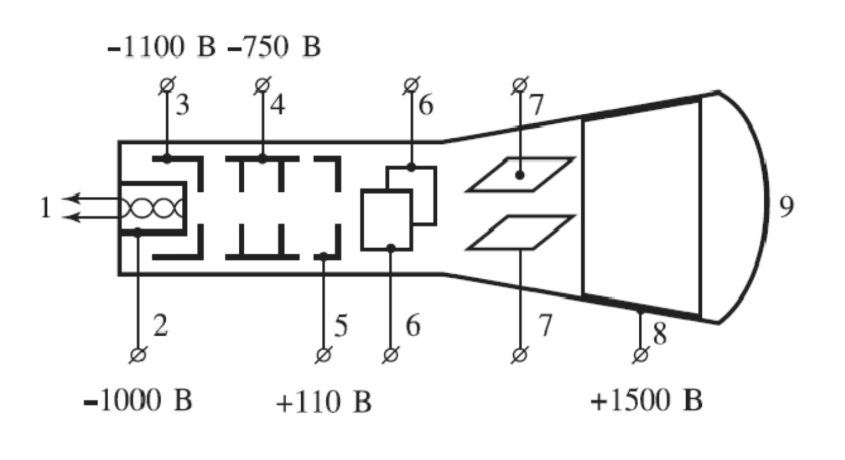
\includegraphics[width=\textwidth]{1}
\end{center}

Здесь $1$ -- подогреватель катода, $2$ -- катод, $3$ -- модулятор, $4$ -- первый (фокусирующий)
анод, $5$ -- второй (ускоряющий) анод, $6$ и $7$ -- горизонтально и вертикально отклоняющие
пластины, $8$ -- третий (ускоряющий) анод, $9$ -- экран.

Электронный пучок формируется системой электродов, называемой "электронной пушкой": катод с нагревателем, модулятор, фокусирующий и ускоряющий аноды. Яркость изображения на экране осциллографа регулируется напряжением на модуляторе (изменяется ручкой "INTEN"), фокус изображения зависит от потенциала первого анода, который можно менять ручкой "FOCUS".

На пути пучка электронов находятся 2 конденстора, электрическое поле в которых взаимно ортогонально, чтобы отклонять пучок в двух взаимных направлениях декартовой системы координат. Регулируя напряжения на конденсаторах, можно определить положения пучка электронов на экране.

\begin{center}
	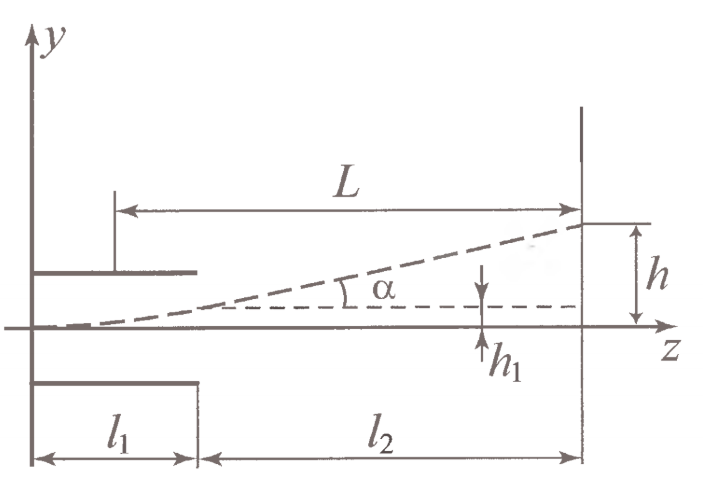
\includegraphics[width=11cm]{2}
\end{center}

Рассматривая движение пучка в электрических полях пластин можно вывести смещение $h$ электронного пятна на экране осциллографа: ${ h =\frac{l_1L}{2dU_\alpha}\cdot U_y}$, где ${ l_1}$ -- длина пластин, ${ L}$ - расстояние от середины пластин до экрана, $d$ -- расстояние между пластинами, ${ U_\alpha} $ -- ускоряющее напряжение на втором аноде.

Чувствительность ЭЛТ к напряжению: ${ k =\frac{l_1L}{2dU_\alpha}}$. Обе последние формулы применимы тогда, когда за время пролёта пучка напряжения на конденсаторах практически не меняется. В итоге получается, что смещение частицы в выбранном направлении прямо пропорционально напряжению на конденсаторе.



Подаваемое на вертикально отклоняющие пластины напряжение должно быть пропорционально самому сигналу:  ${ U_y(t) = U_{0y}+k_{yu}U_c(t).}$\\
${ U_{0y}}$ -- постоянное напряжение, определяющие расположение графика сигнала по оси $Y$; ${ k_{uy}}$ -- коэффициент входного сигнала каналом вертикального отклонения.

Подаваемое на горизонтально отклоняющие пластины напряжение должно линейно зависить от времени : ${ U_x = U_{0x}+ k_{xu}t}$, где ${ U_{0x}}$ -- постоянное напряжение, определяющие расположение графика сигнала по оси $Х$; ${ k_{xu}}$ -- коэффициент пропорциональности, зависящий от рабочих харрактеристик генератора развертки и усилителя.

Напряжение пилообразной формы, вырабатываемое генератором развёртки осциллографом, изображено на рисунке. Во время прямого хода луч проходить через весь экран слева направо, после чего напряжение сбрасывается во время обратного хода. Далее после времени ожидания снова появляется луч на экране. Общее время ожидания и обратного хода называется временем блокировки.

\begin{center}
	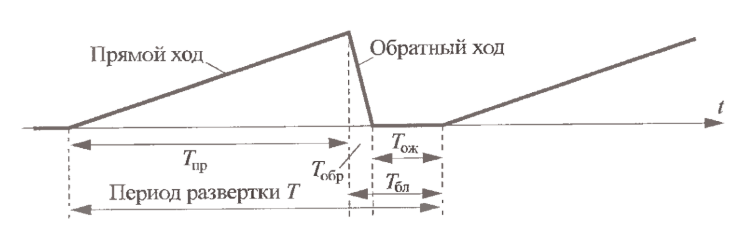
\includegraphics[width=14cm]{3}
\end{center}

При наблюдении периодических быстропротекающих процессов важно зафиксировать изображение на экране, для чего используется синхронизация: для неподвижного изображения необходимо, чтобы период развёртки был кратен периоду излучаемого сигнала, что можно сделать, "навязав" свой период генератору развёртки (для генератора развёртки есть несколько режимов на осциллографе).

\section{Ход работы}

\subsection{Наблюдение периодического сигнала от генератора и
измерение его частоты}

Настроим осциллограф на работу, выставив все нужные параметры на ручках и кнопках (см. приложение работы осциллографа GOS-620).

Подключим звуковой генератор в каналу $CH2$, выставив частоту на генераторе $f_{\text{ЗГ}} = 1$ кГц, и получим на экране устойчивую картину колебаний.

Измерим период наблюдаемого сигнала для заданной частоты, далее проделываем то же самое для других значений частот звукового генератора:
\begin{center}
\begin{tabular}{|c|c|c|c|c|c|c|}
\hline 
$f_{\text{ЗГ}}$, кГц & $T$, дел & мc/дел & $T$, мс & $f$, кГц & $\delta f$, кГц & $f - f_{\text{ЗГ}}$, кГц  \\ 
\hline 
0,01 & 5 & 20 & 100 & 0,01 & 0,0004 & 0 \\ 
\hline 
0,05 & 5 & 4 & 20 & 0,05 & 0,002 & 0 \\ 
\hline 
0,1 & 5 & 2 & 10 & 0,1 & 0,004 & 0 \\ 
\hline 
1 & 5 & 0,2 & 1 & 1 & 0,04 & 0 \\ 
\hline 
10 & 5 & 0,02 & 0,1 & 10 & 0,4 & 0 \\ 
\hline 
100 & 5 & 0,002 & 0,01 & 100 & 4 & 0 \\ 
\hline 
1000 & 5 & 0,0002 & 0,001 & 1000 & 40 & 0 \\ 
\hline 
10000 & 5 & 0,00002 & 0,0001 & 10000 & 400 & 0 \\ 
\hline 
\end{tabular}
\end{center}

Погрешности частот найдены по следующим формулам:
\[ \delta f = \frac{\delta T}{T^2},\text{ где } \delta T = 0,2 \cdot \text{[мc/дел]}\]

\subsection{Измерение амплитуды сигнала}

Для начала измерим максимальную и минимальную амплитуды напряжений от генератора:
\[U_{min} = 0,004 \text{ В, } U_{max} = 20 \text{ В}\]

Выразим отношение максимального и минимального уровней сигнала в децибелах [дБ]:
\[\beta = 10 \cdot lg \frac{P_2}{P_1} = 20 \cdot lg \frac{U_2}{U_1} = 20 \cdot lg \frac{U_{max}}{U_{min}} = 73,98 \text{ [дБ]}\]

Здесь было учтено, что средняя мощность попрорциональная амплитуде в квадрате: $P\sim U^2$.

\subsection{Измерение амплитудно-частотной характеристики осциллографа}

Амплитудо-частнотной характеристикой (АЧХ) измерительного прибора называют зависимость амплитуды измеряемого
сигнала от частоты сигнала, подаваемого на вход.

Установим частоту сигнала генератора $f = 1$ кГц и получим
устойчивое изображение синусоиды на экране. Подберём масштаб вертикальной шкалы осциллографа так, чтобы размах (удвоенная амплитуда) сигнала на
экране составил $2U_0 = 4,0$ дел и далее не будем его менять.

Будем изменять частоту генератора во всём возможном диапазоне измерений, исследуя зависимость отношение амплитуды сигнала на осциллографе $U(f)$ к исходной $U_0$ в зависимости от частоты:
\[K(f) = \frac{U(f)}{U_0}\]
 
Составим таблицу для открытого сигнала $DC$:
\begin{center}
\begin{tabular}{|c|c|c|c|c|c|c|c|c|c|c|}
 \hline 
 $\frac{U}{U_0}$ & 1 & 1 & 1 & 0,96 & 0,96 & 0,92 & 0,88 & 0,84 & 0,80 & 0,76 \\ 
 \hline 
 $f$, МГц & 0,05 & 0,2 & 0,5 & 0,7 & 2 & 6 & 7 & 9 & 10,1 & 12 \\
 \hline 
 $lgf$ & 4,70 & 5,3 & 5,70 & 5,845 & 6,32 & 6,78 & 6,845 & 6,954 & 7 & 7,08 \\  
 \hline 
 $\frac{U}{U_0}$ & 0,68 & 0,64 & 0,6 & 0,56 & 0,52 & 0,48 & 0,44 & 0,4 & 0,36 & 0,32 \\ 
 \hline 
 $f$, МГц & 13 & 15 & 16 & 17,5 & 19,8 & 21,1 & 22,5 & 24,2 & 26,3 & 28,5 \\ 
 \hline
 $lgf$ & 7,11 & 7,176 & 7,2 & 7,24 & 7,30 & 7,324 & 7,35 & 7,38 & 7,42 & 7,455 \\  
 \hline  
 \end{tabular}
 \end{center}
  
Заметим, что при очень низких частотах отношения напряжений равно единице, поэтому в таблицу такие данные мы не записали. 

Теперь составим таблицу для закрытого сигнала $AC$:\\

\begin{tabular}{|c|c|c|c|c|c|c|c|c|c|c|}
 \hline 
 $\frac{U}{U_0}$ & 1 & 1 & 1 & 1 & 0,96 & 0,92 & 0,88 & 0,84 & 0,80 & 0,76 \\ 
 \hline 
 $f$, МГц & 0,05 & 0,2 & 0,5 & 1,5 & 3 & 6 & 7,4 & 9 & 10,4 & 12 \\ 
 \hline
 $lgf$ & 4,70 & 5,3 & 5,70 & 6,18 & 6,48 & 6,78 & 6,87 & 6,954 & 7,02 & 7,08 \\  
 \hline 
 $\frac{U}{U_0}$ & 0,68 & 0,64 & 0,6 & 0,56 & 0,52 & 0,48 & 0,44 & 0,4 & 0,36 & 0,32 \\ 
 \hline 
 $f$, МГц & 14,9 & 16,2 & 16,7 & 17,5 & 18,8 & 20 & 21,3 & 22,6 & 23,8 & 25,1 \\ 
 \hline 
 $lgf$ & 7,17 & 7,21 & 7,22 & 7,24 & 7,27 & 7,3 & 7,33 & 7,35 & 7,37 & 7,40 \\  
 \hline
 \end{tabular}
 
\textbf{ }

Построим в единых осях графики зависимостей коэффициента ослабления сигнала от частоты -- графики практически совпадают.

\begin{center}
	\includegraphics[width=13cm]{15}
\end{center}

Возможное различие в режимах -- присутствие конденсатора в закрытом режиме сигнала для ослабления постоянной составляющей напряжения.\\


\subsection{Изучение влияния АЧХ на искажение сигнала}

Переключим режим сигнала с синусоидального на прямоугольные импульсы -- миандры. Частоту генератора будем менять в широком диапазоне частот.

Для открытого сигнала получим следующие картины на экране:
\[f = 50 \text{ Гц}\]

\begin{center}
	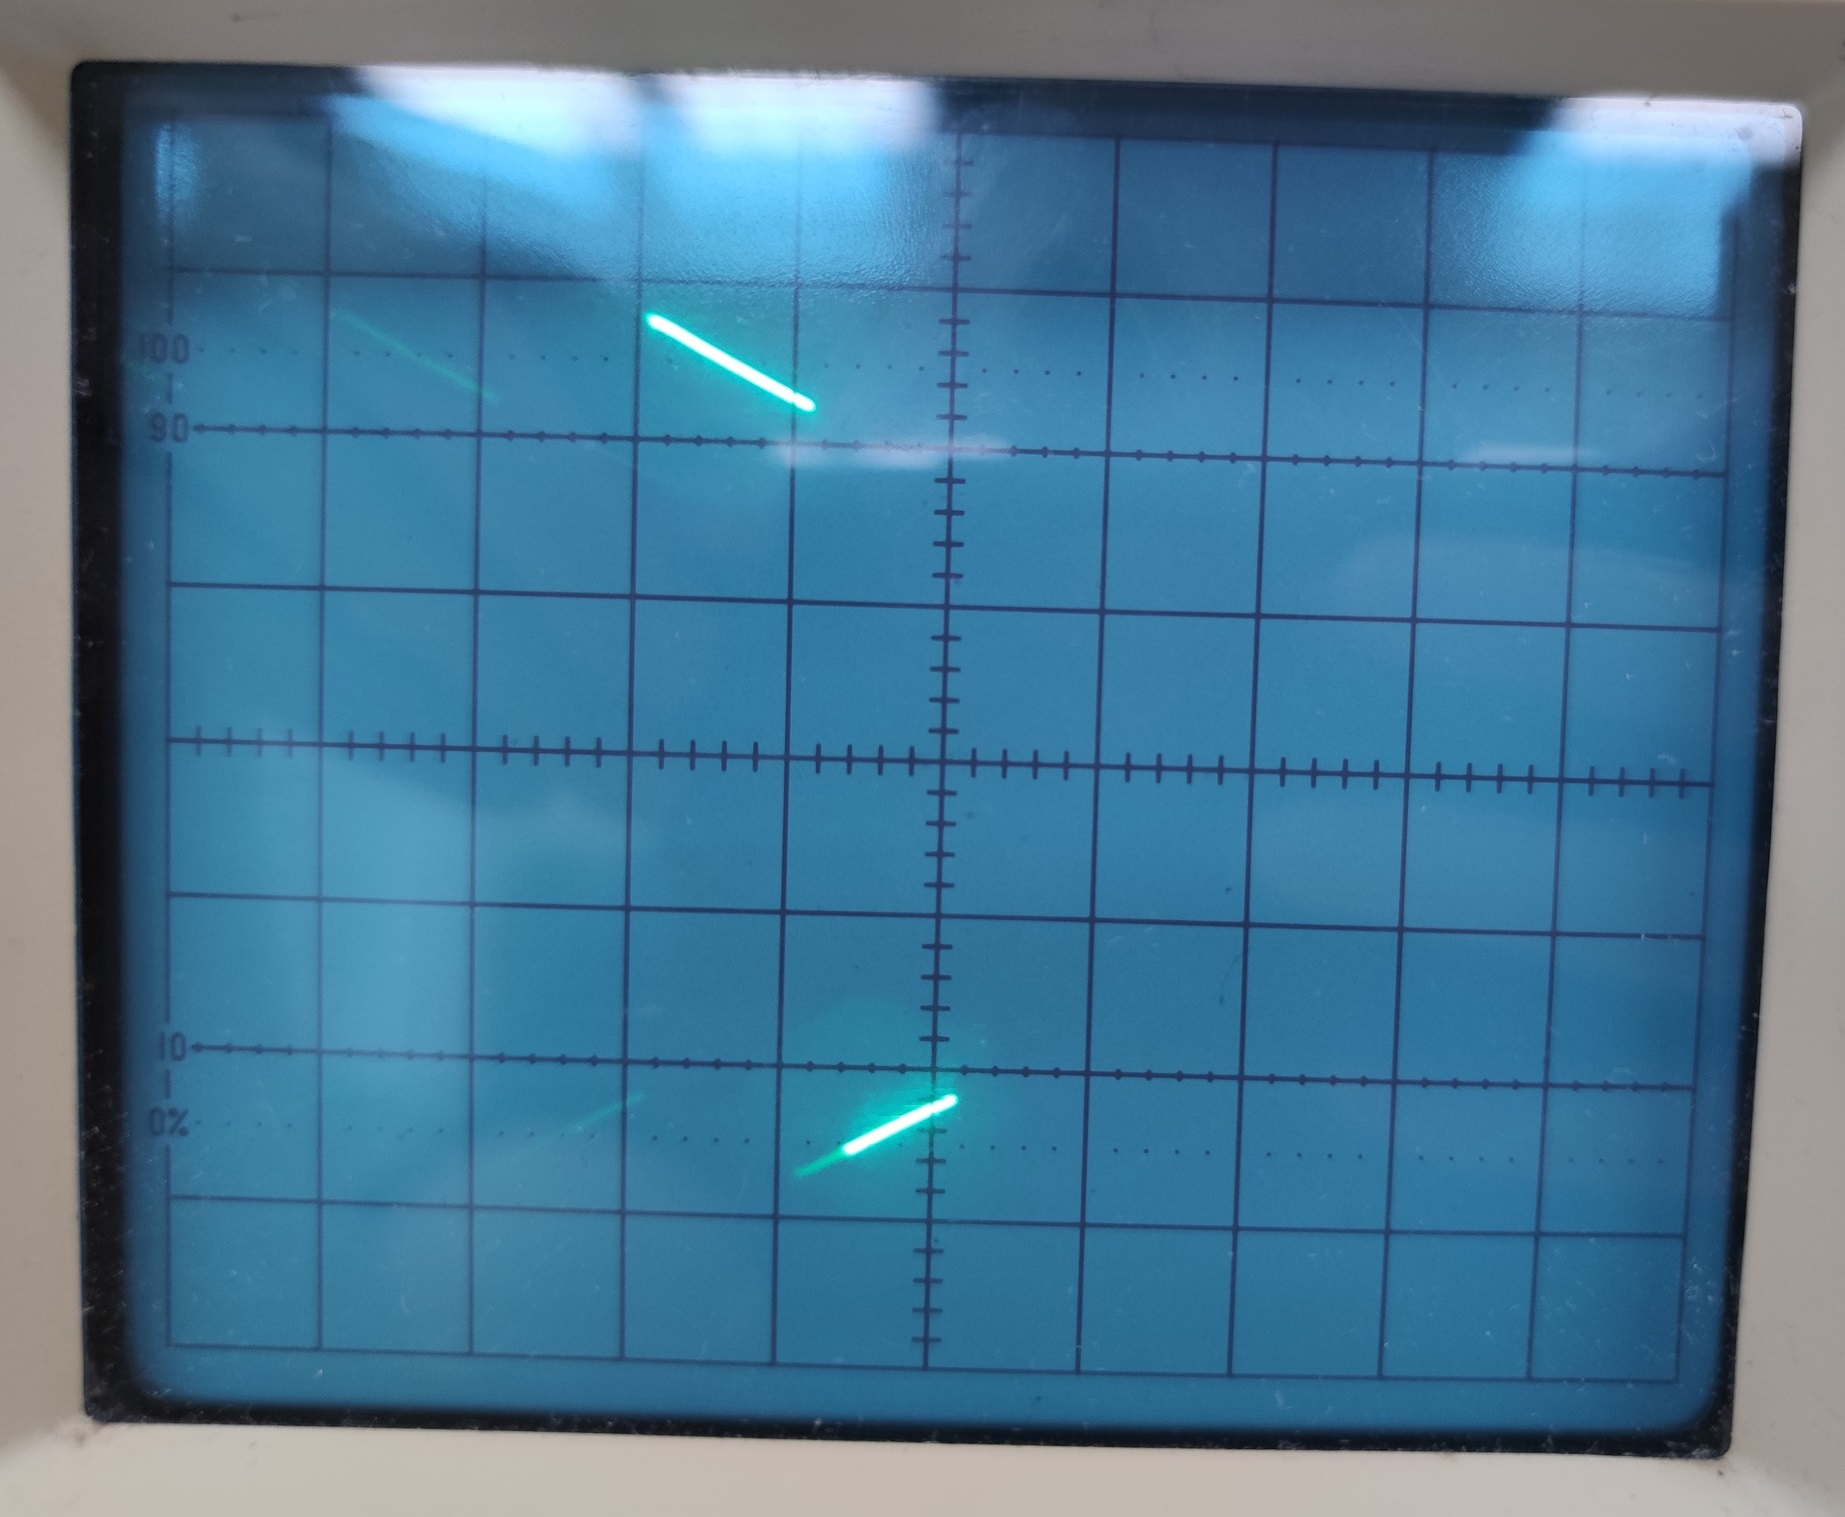
\includegraphics[width=7cm]{4}
\end{center}

\[f = 10 \text{ кГц}\]

\begin{center}
	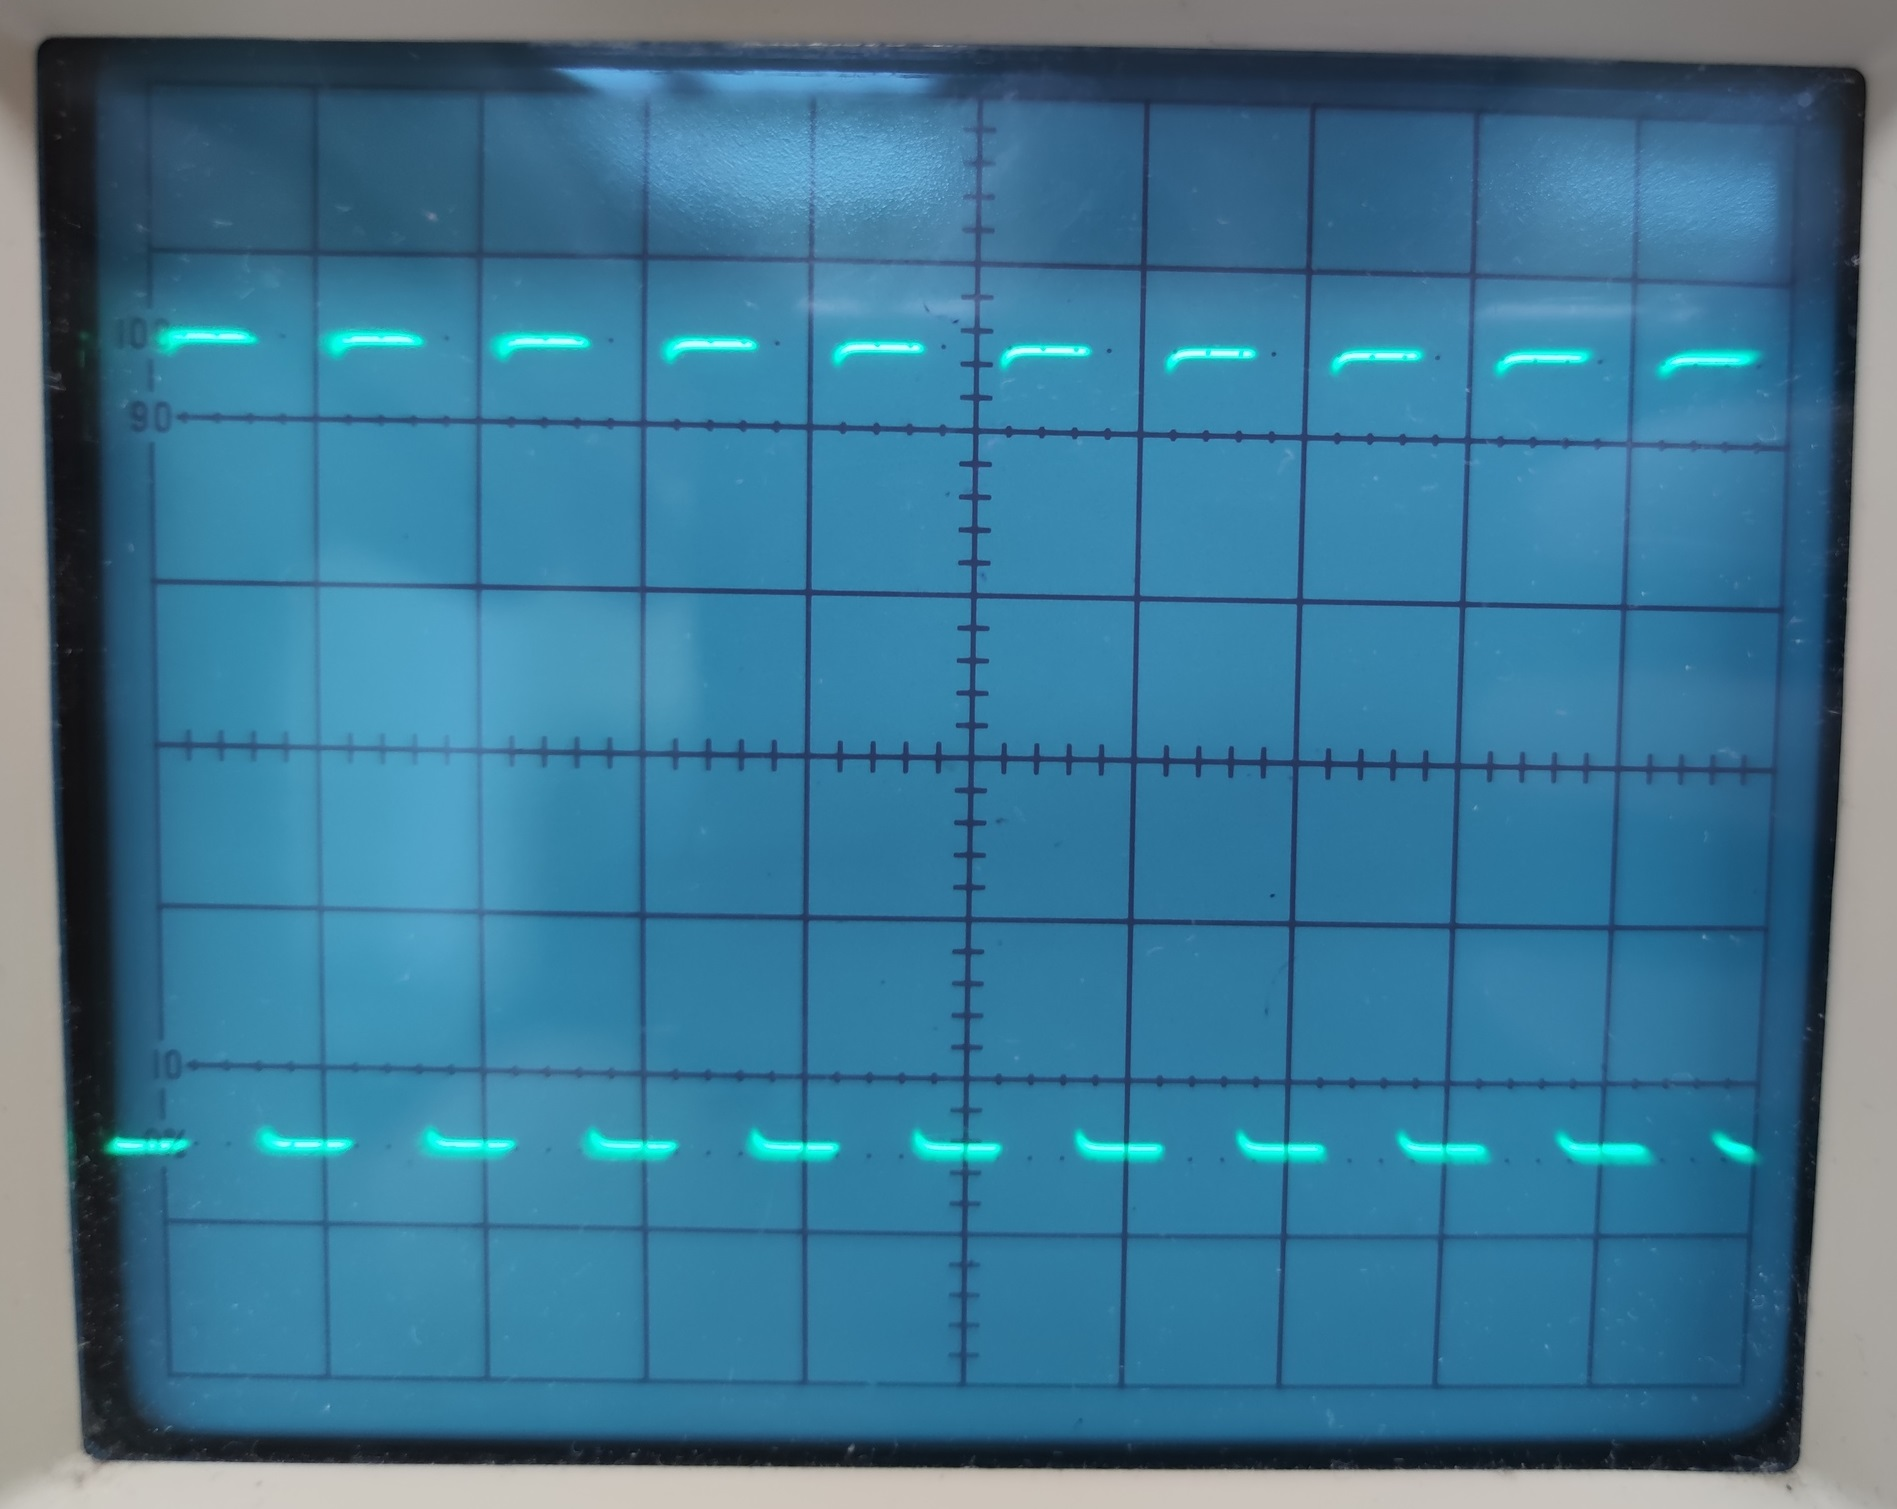
\includegraphics[width=10cm]{5}
\end{center}

\[f = 100 \text{ кГц}\]

\begin{center}
	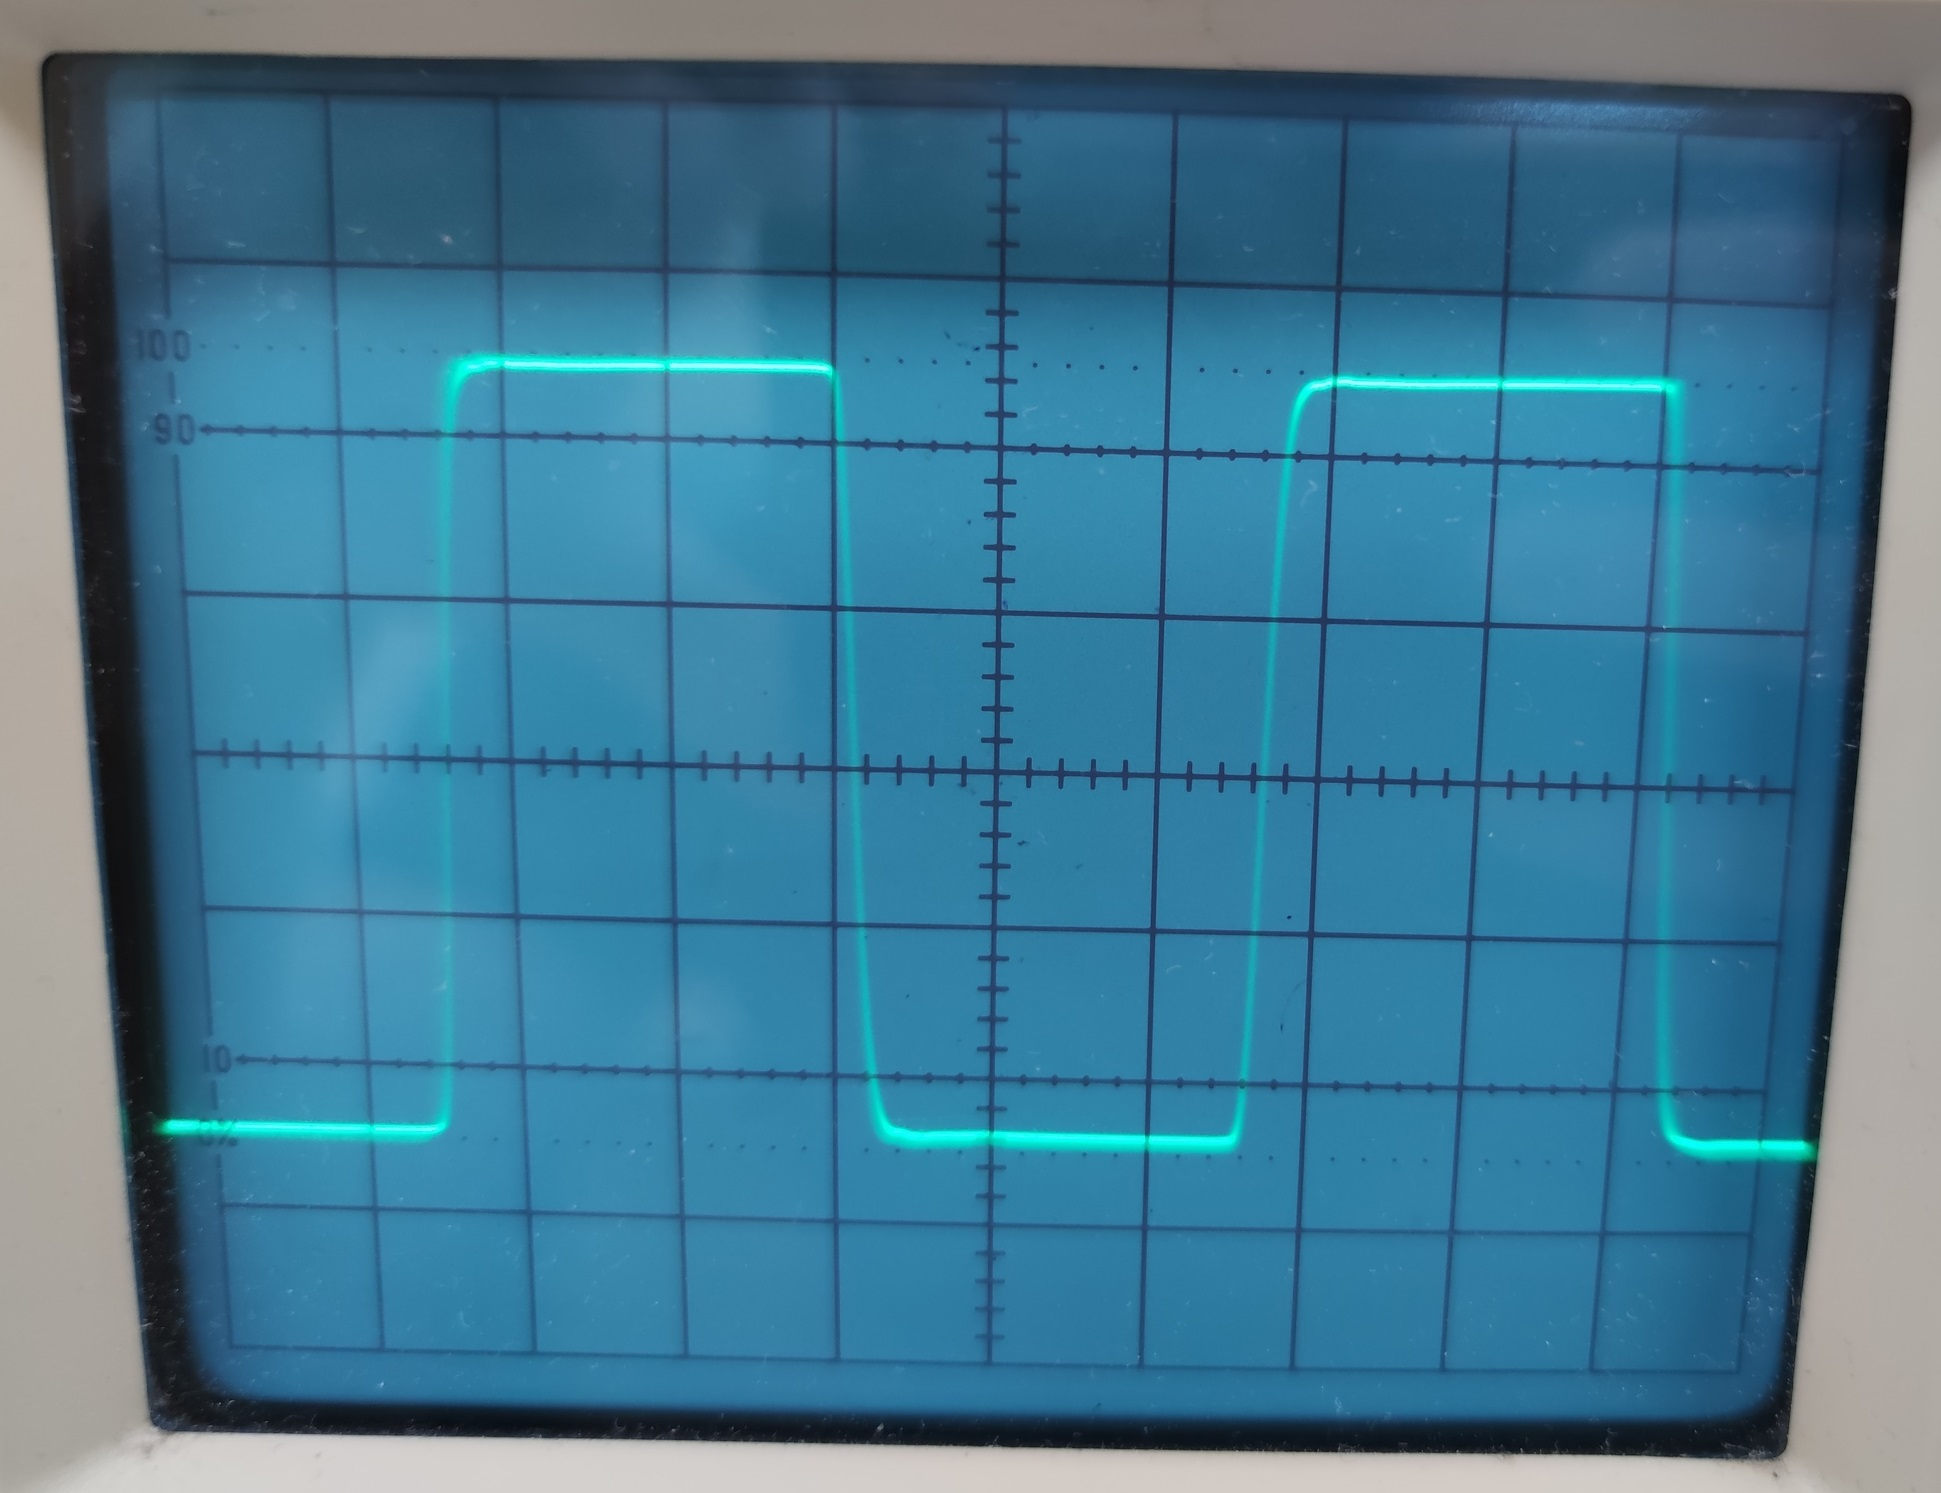
\includegraphics[width=10cm]{6}
\end{center}

\newpage
\[f = 1 \text{ МГц}\]
\begin{center}
	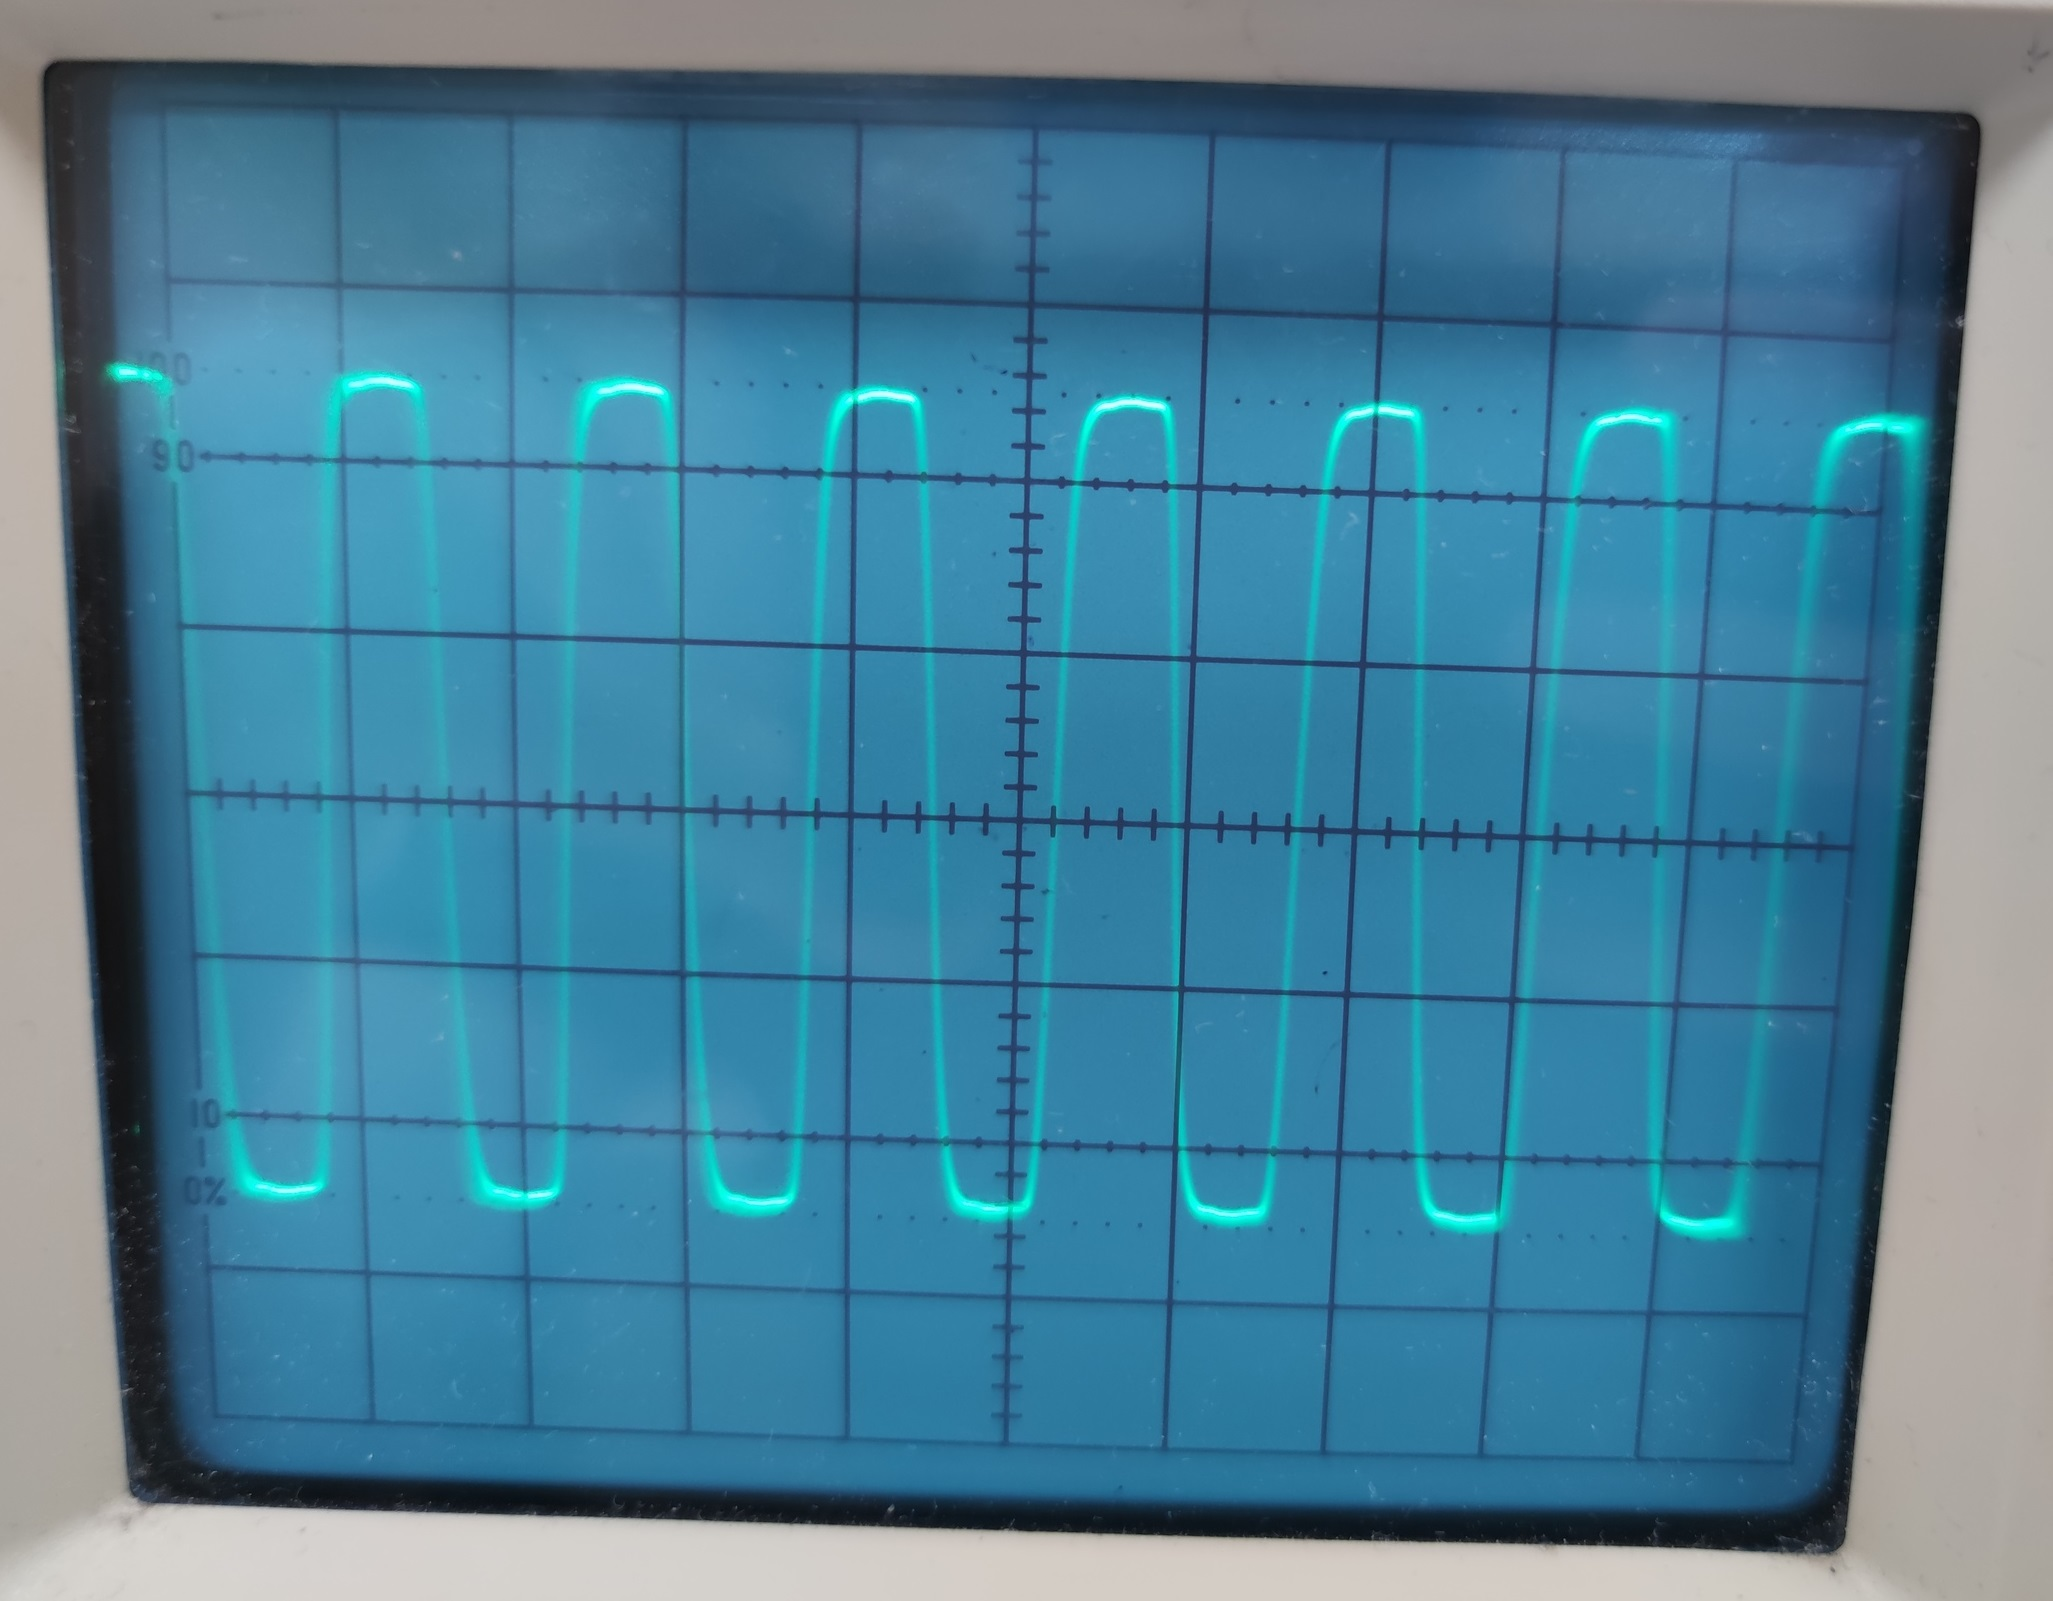
\includegraphics[width=9cm]{7}
\end{center}

\[f = 5 \text{ МГц}\]
\begin{center}
	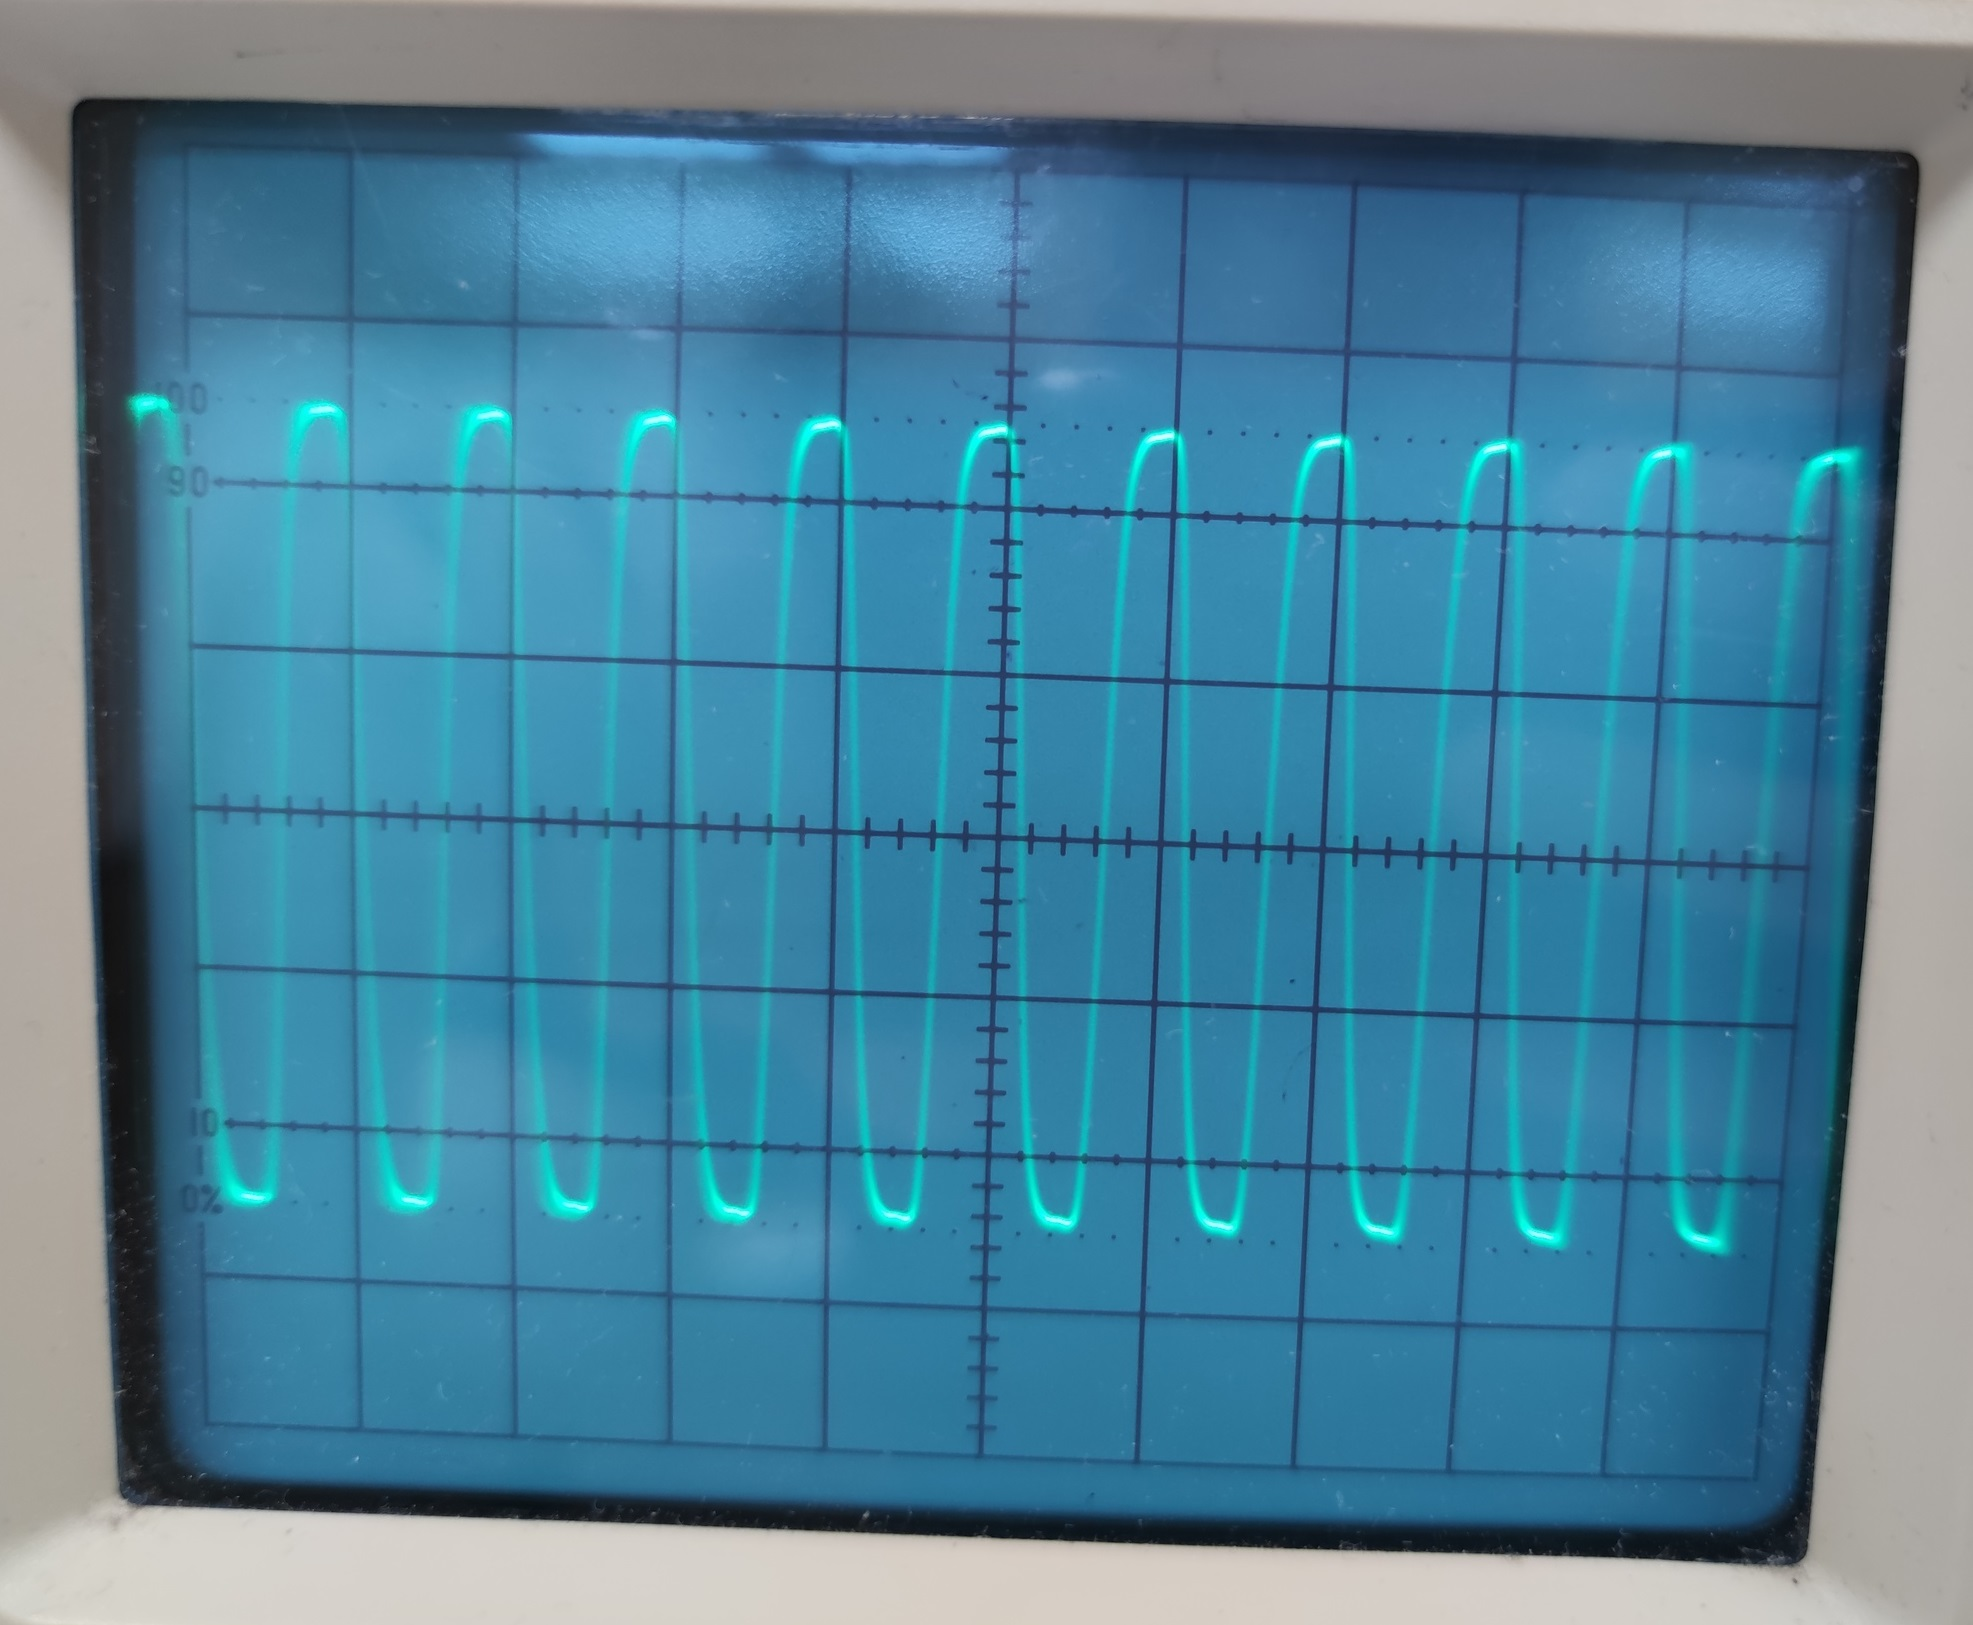
\includegraphics[width=9cm]{8}
\end{center}

Можно заметить, что наибольшие искажения наблюдаются при очень малых и больших частотах. 
Причинами искажения формы сигнала могут быть неудовлетворительные амплитудные и фазочастотные карактеристики усилителей и делителей напряжения, неравномерная развертка, а также сама электроннолучевая трубка. Искажение осциллограмм может также вызываться внешними электрическими и магнитными полями, в частности полями электрической сети. 

Кроме неизбежных искажений осциллограмм, вызываемых влиянием емкости пластин и подводящих проводов, качество воспроизведения осциллограмм в значительной мере зависит от схемы включения электроннолучевой трубки.

Картины для закрытого входа имеют примерно тот же вид.

\subsection{Измерение разности фазово-частотных характеристик
каналов осциллографа}

Фазово-частотной характеристикой
(ФЧХ) называют зависимость разности фаз входного и выходного
сигналов от частоты. Осциллограф может быть использован для
измерения разности фаз между подаваемыми на него сигналами, при
этом однако необходимо учитывать, что каналы $X$ и $Y$ могут иметь
разные ФЧХ.

Измерим разность фаз, возникающую при подаче одного и того же сигнала на разные каналы осциллографа, в зависимости от частоты сигнала.

Зафикисируем частоту генератора $f = 1$ кГц, подадим синусоидальный сигнал через разветвлитель сразу на два каналм $CH1$ и $CH2$.

Выключим внутреннюю развертку осциллографа, переведя переключатель $TIME/DIV$ в положение $X - Y$. В этом режиме отклонение луча на экране пропорционально подаваемым на каналы напряжениям $Y(t) = k_y U_y (t)$, $X(t) = k_x U_x (t)$, где коэффициенты
масштаба $kx$, $ky$ определяются положениями ручек $VOLTS/DIV$.

Установим переключатели режимов каналов $X$ и $Y$ в положение $GND$ (выключены) и ручками $POSITION$ установим точку в центр экрана. После этого установим переключатели режимов каналов $X$ и $Y$ в положения $AC$ (закрытые входы). Используя ручки
$VOLTS/DIV$ обоих каналов, получим на экране отрезок прямой
(вырожденный эллипс) под углом $45^{\circ}$ к горизонтали, занимающий
большую часть экрана.

Изменяя частоту генератора $f$ во всем доступном диапазоне найдём участки, на которых изображение на экране переходит из отрезка в невырожденный эллипс. На этих участках проведём подробное измерение разности фаз $ \varphi (f)$ между каналами $X$ и $Y$ в
зависимости от частоты.

При подаче на взаимно перпендикулярные отклоняющие пластины двух синусоидальных сигналов траектория луча на экране
осциллографа представляет собой эллипс и может быть в общем
виде описана уравнениями
\[x(t) = A_x sin(\omega t + \varphi_x), \text{ } y(t) = A_y sin(\omega t + \varphi_y)\]

Из этих формул нетрудно получить разность фаз (см. картину):
\[|\Delta \varphi| = arcsin | \frac{y_0}{A_y}| \text{, или } |\Delta \varphi| = \pi - arcsin | \frac{y_0}{A_y}|\]

Занесём все измеренные данные в таблицу и построим на их основе график зависимости $\varphi (lgf)$ с учётом того, что по условию достаточно определить только модуль разности фаз:

\begin{center}
\begin{tabular}{|c|c|c|c|c|c|c|c|c|c|}
\hline 
$f$, кГц & 80 & 300 & 500 & 680 & 870 & 1100 & 1500 & 1700 & 2100  \\ 
\hline 
$lgf$ & 4,9 & 5,48 & 5,7 & 5,83 & 5,94 & 6,04 & 6,18 & 6,23 & 6,32  \\ 
\hline 
$|2y_0|$, В & 0,4 & 0,8 & 1,2 & 1,6 & 2,2 & 2,8 & 3,5 & 4 & 4,2   \\ 
\hline 
$|2A_y|$, В & 5 & 5 & 5 & 4,8 & 4,6 & 4,6 & 4,4 & 4,2 & 4,2 \\ 
\hline 
$\Delta \varphi$ & 0,08 & 0,16 & 0,24 & 0,34 & 0,50 & 0,65 & 0,92 & 1,26 & 1,57  \\
\hline 
$arcsin | \frac{y_0}{A_y}|$ & 0,08 & 0,16 & 0,24 & 0,34 & 0,50 & 0,65 & 0,92 & 1,26 & 1,57  \\ 
\hline 
\end{tabular} 
\end{center}

\begin{center}
	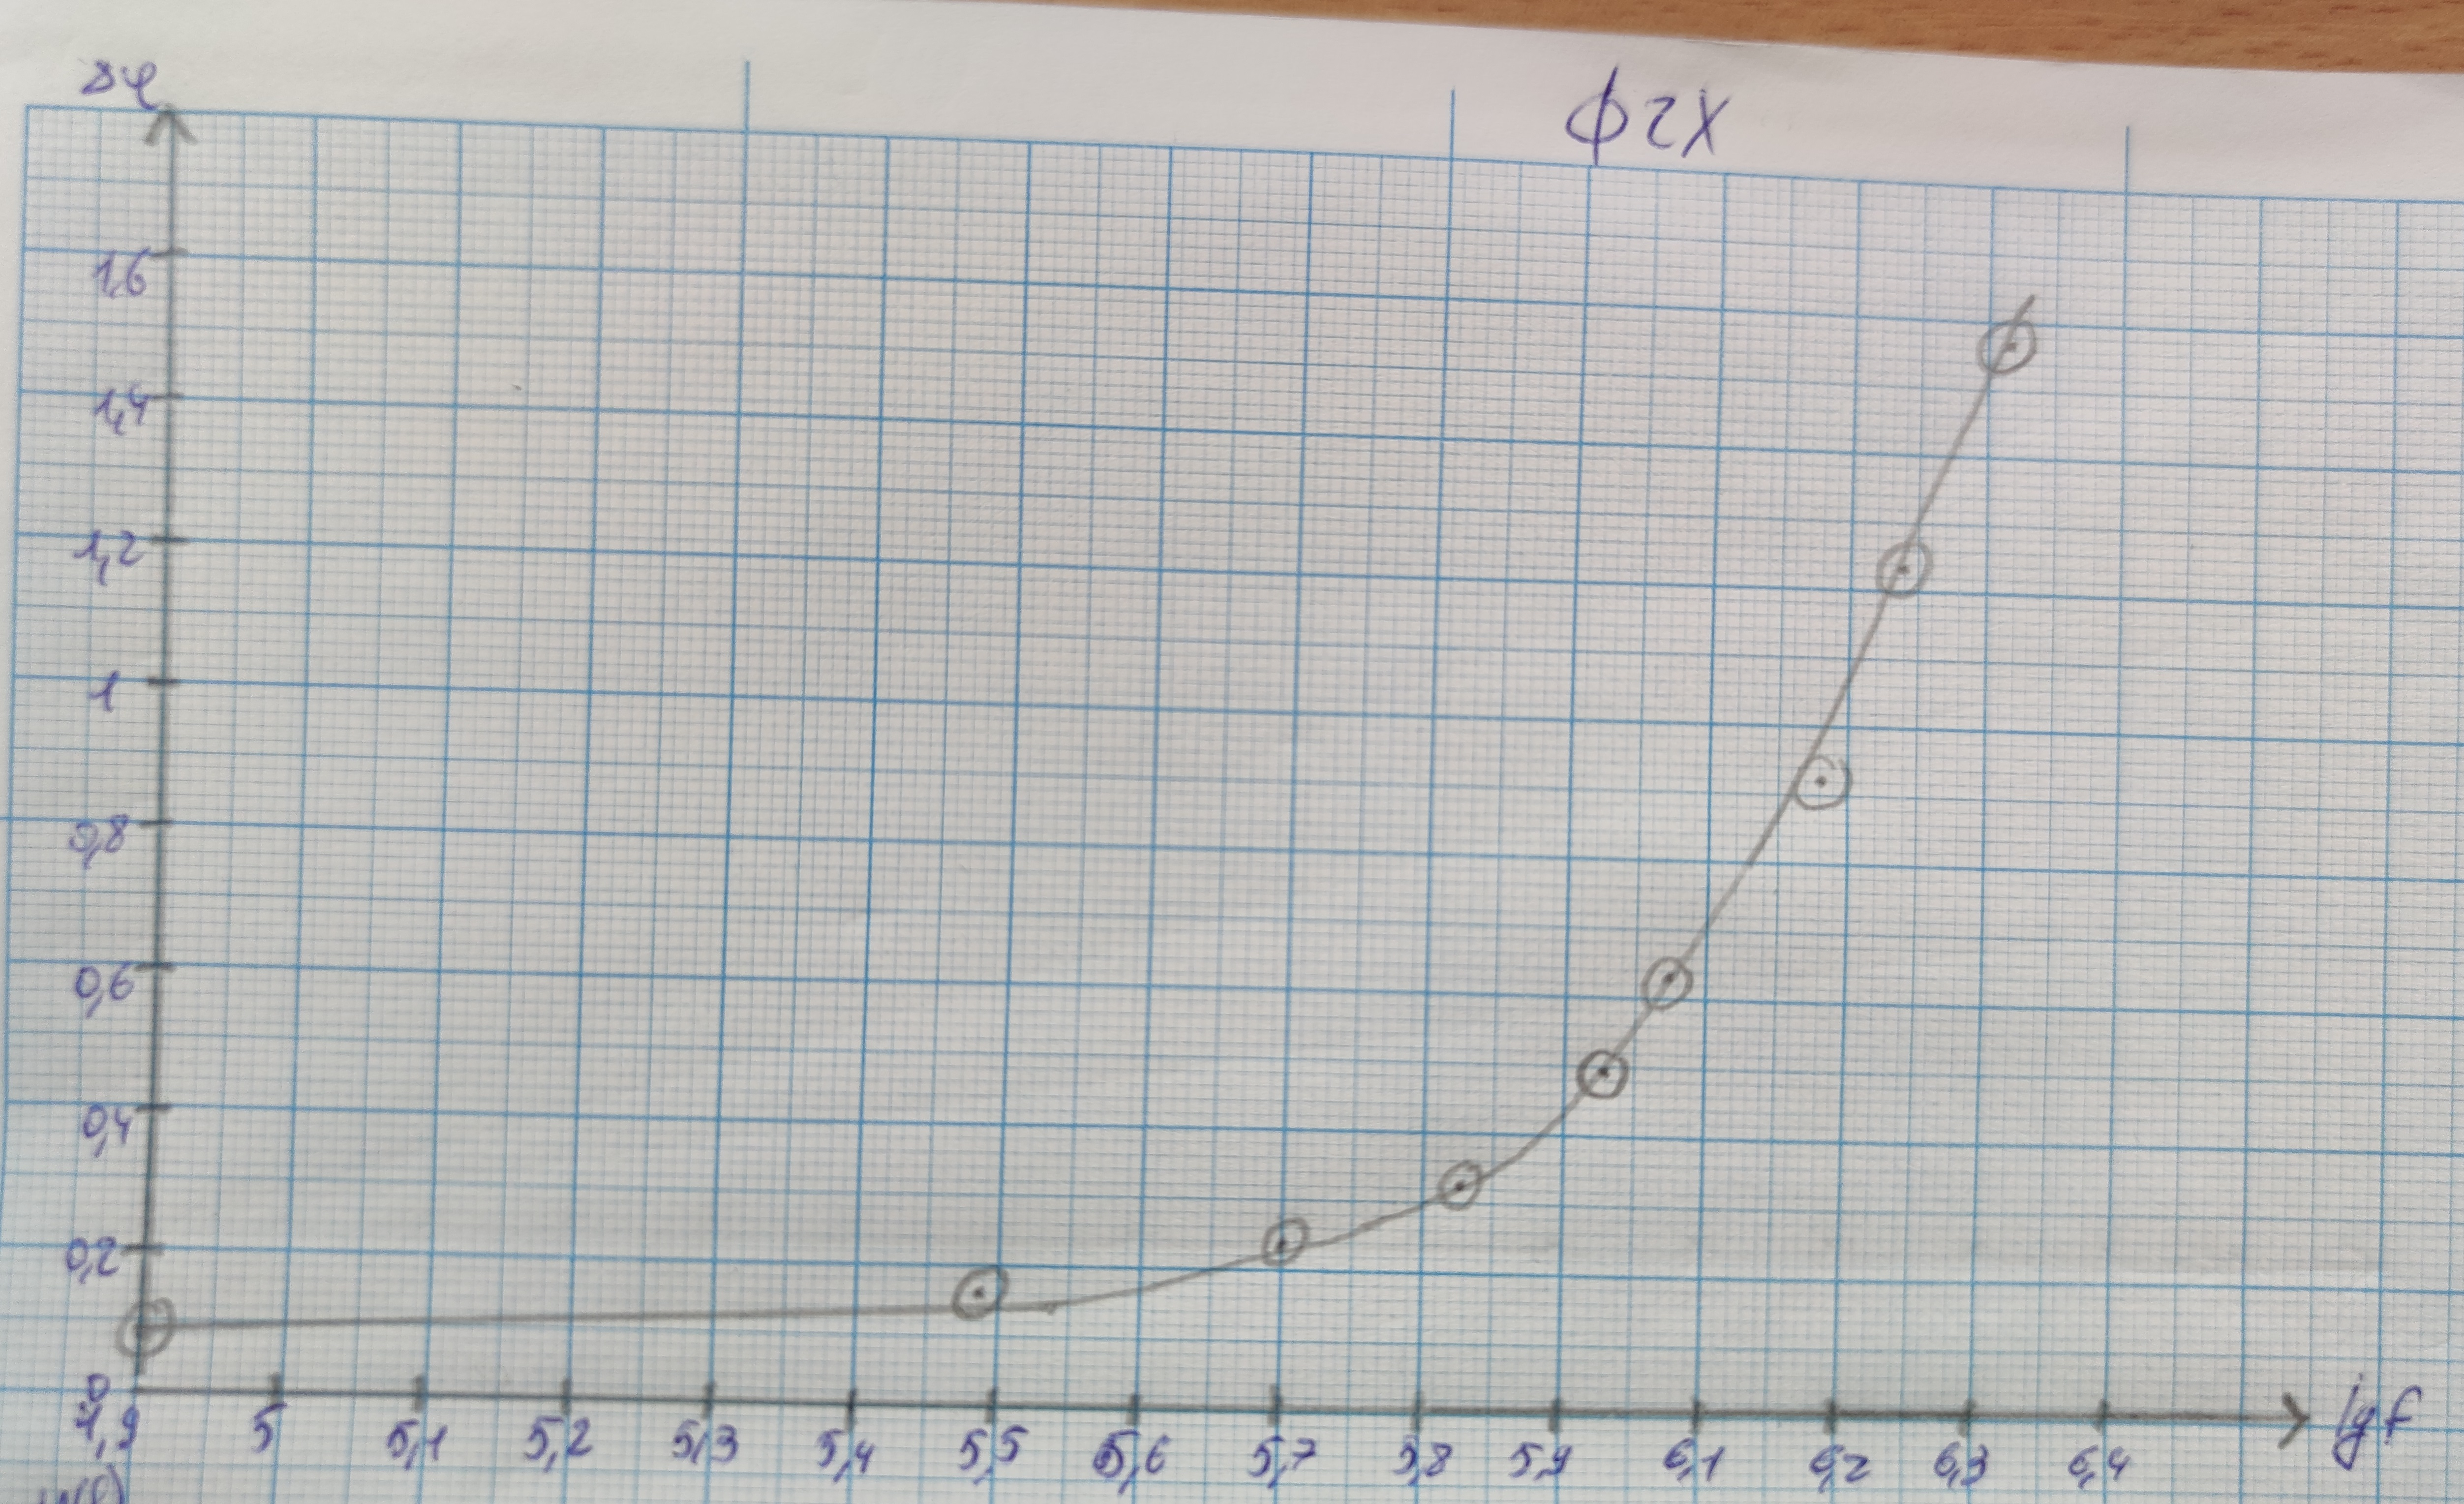
\includegraphics[width=14cm]{13}
\end{center}

При низких частотах наблюдать разность фаз невозможно, так как эллипс остаётся вырожденным и расстояния нельзя посчитать. Поэтому разность фаз можно наблюдать только начиная с частот порядка $10$ кГц.


\subsection{Наблюдение фигур Лиссажу и измерение частоты}

Подадим на вход каналов $X$ и $Y$ осциллографа сигналы с двух разных звуковых генераторов. Установим приблизительно одинаковые частоты генераторов. Амплитуды генераторов и положения ручек $VOLTS/DIV$ осциллографа установим
таким образом, чтобы фигура Лиссажу занимала большую часть
экрана, не выходя за его пределы.

Изменяя $f_x$, получим устойчивые фигуры для нескольких целочисленных отношений частот.

\begin{center}
	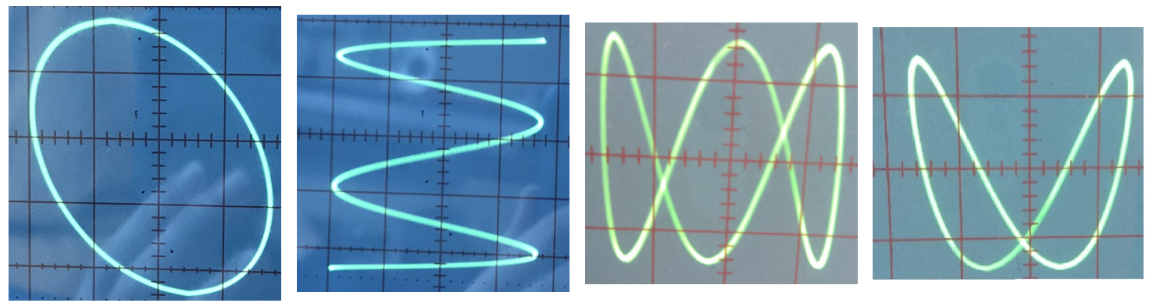
\includegraphics[width=14cm]{11}
\end{center}

На рисунках приведены фигуры Лиссажу со следующими отношениями частот соответственно: $1 : 1$, $1 : 5$, $3 : 1$, $2 : 1$.

Определить отношение частот по фигуре Лиссажу можно следующим способом: проводим такие вертикальную и горизонтальную линии через фигуру, чтобы количество пересечений этих линий с фигурой было максимальным и считаем количество пересечений этих пересечений. Так как сигналы изменяются гармонически, то количество пересечений определяются периодом сигнала, значит и частотой сигнала.\\

\text{ }

\subsection{Измерение АЧХ интегрирующей и дифференцирующей RC-цепочек}

Измерим амплитудно-частотные характеристики $RC$ цепочек, представленных на схемах:

\begin{center}
	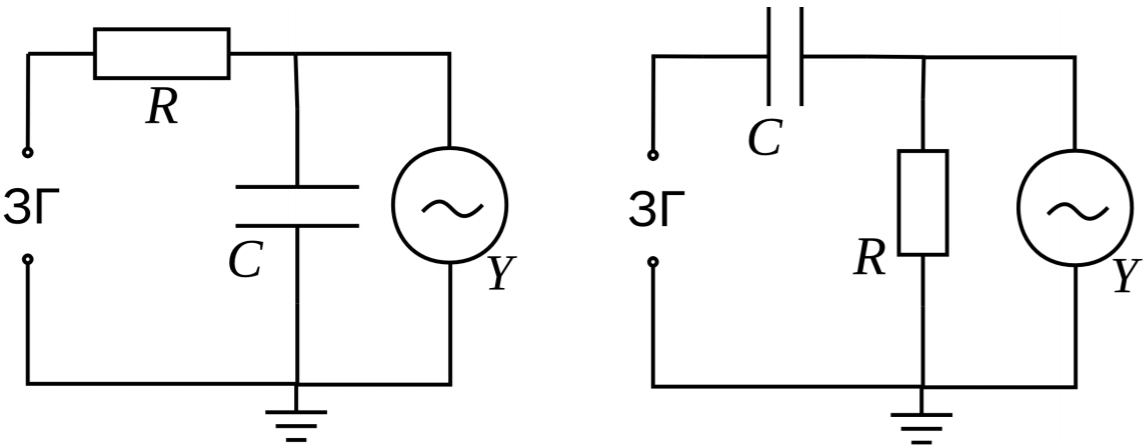
\includegraphics[width=12cm]{12}
\end{center}

Сопротивление реостата в схемах равно $3$ кОм, ёмкость конденсатора равна $0,01$ мкФ. Для удобства посчитаем величину $\tau = RC = 0,03$ мс. 

Теоретически АЧХ таких схем описываются формулами:

\[\frac{U(f)}{U_0} = \frac{1}{\sqrt{(\omega \tau)^2 + 1}},\text{ } \frac{U(f)}{U_0} = \frac{1}{\sqrt{(\omega \tau)^{-2} + 1}}\]

Запишем измеренные данные АЧХ в таблицу вместе с теоретическими данными:

Интегрирующая цепочка:
\begin{center}
\begin{tabular}{|c|c|c|c|c|c|c|c|c|c|c|}
 \hline 
 $\frac{U}{U_0}$ & 1 & 0,96 & 0,92 & 0,88 & 0,84 & 0,80 & 0,76 & 0,72 & 0,68 & 0,60\\ 
 \hline 
 $\frac{U}{U_0} \text{(теор)}$ & 1 & 0,962 & 0,924 & 0,884 & 0,842 & 0,80 & 0,755 & 0,714 & 0,675 & 0,59\\
 \hline 
 $f$, кГц & 0,01 & 1,5 & 2,2 & 2,8 & 3,4 & 4 & 4,6 & 5,2 & 5,8 & 7,2 \\ 
 \hline 
 $\frac{U}{U_0}$  & 0,52 & 0,44 & 0,36 & 0,28 & 0,20 & 0,12 &&&&  \\ 
 \hline 
 $\frac{U}{U_0} \text{(теор)}$  & 0,503 & 0,425 & 0,34 & 0,26 & 0,18 & 0,10 &&&&  \\ 
 \hline 
 $f$, кГц & 9,1 & 11,3 & 14,6 & 19,5 & 29 & 53 &&&& \\ 
 \hline 
 \end{tabular}
 \end{center}
 

Дифференцирующая цепочка:
\begin{center}
\begin{tabular}{|c|c|c|c|c|c|c|c|c|c|c|}
 \hline 
 $\frac{U}{U_0}$ & 1 & 0,96 & 0,92 & 0,88 & 0,84 & 0,80 & 0,76 & 0,72 & 0,68 & 0,60\\ 
  \hline 
 $\frac{U}{U_0} \text{(теор)}$ & 1 & 0,955 & 0,91 & 0,86 & 0,816 & 0,775 & 0,738 & 0,70 & 0,655 & 0,582\\
 \hline 
 $f$, кГц & 100 & 17 & 12 & 9 & 7,5 & 6,5 & 5,8 & 5,2 & 4,6 & 3,8 \\ 
 \hline 
 $\frac{U}{U_0}$  & 0,52 & 0,44 & 0,36 & 0,28 & 0,20 & 0,12 &&&&  \\ 
 \hline 
 $\frac{U}{U_0} \text{(теор)}$  & 0,49 & 0,41 & 0,337 & 0,255 & 0,185 & 0,103 &&&&  \\ 
 \hline 
 $f$, кГц & 3 & 2,4 & 1,9 & 1,4 & 1 & 0,6 &&&& \\ 
 \hline 
 \end{tabular}
 \end{center}
 
\begin{center}
	\includegraphics[width=14cm]{14}
\end{center}
 
 На основе данных, занесённых в таблицу, строим экспериментальные и теоретические графики. Видно, что теоретические и экспериментальные зависимости почти совпадают, значит формулы для амлитуды справедливы (на графике их тяжело различить, поэтому через теоретические и экспериментальные графики проведена одна аппроксимирующая прямая).


\section{Выводы}

В результате знакомились с устройством и принципом работы осциллографа GOS-620, изучили его основные характеристики. Также научились пользоваться генератором звуковых частот, исследовали искажения изображений на экране осциллографа при больших частотах, научились наблюдать фигуры Лиссажу а также исследовали амплитудно-частотные характеристики интегрирующей и дифференцирующей $RC$ цепочек.




\end{document}